\documentclass[twoside,a4paper]{book}
\usepackage{fricas}

\begin{document}
%
% \thispagestyle{empty}
% \vspace*{1in}
% {\Large\sf Richard D. Jenks \hfill Robert S. Sutor \newline
% \vskip 1in
% \begin{center}
% \LARGE\sf AXIOM \\
% \quad \\ \quad \\
% \Large\sf The Scientific Computation System
% \quad \\ \quad \\ \vskip 1.5in
% \normalsize\rm Draft: \today
% \end{center}}
% \newpage
% \thispagestyle{empty}
% \quad
%
\pagenumbering{roman}
\setcounter{page}{0}

\begin{quote}
\color{red}\Large
  This is an attempt to make the content of the Axiom book (by Jenks
  and Sutor) available again in order to describe the FriCAS project
  (which is a fork of the original Axiom code). The following
  material is mainly taken from the original Axiom book, but is partly
  tailored to new developments in FriCAS.

  \vspace{1cm}

  \textbf{WARNING: This is work-in-progress! There might be errors and
    even false statements.}

  Plan is as follows:
  \begin{enumerate}
  \item Make LaTeX compilation work and include (generated) pictures
    and generated output of algebra commands.
  \item Simplify and remove redundant \LaTeX{} commands.
  \item Build on modern advanced latex packages.
  \item Generate indices and hyperrefs.
  \end{enumerate}

  All of the above will be done by taking care of still generating the
  same \texttt{.ht} files although the technicalities might look
  different. The contents of the files (no matter how wrong it
  actually is) will only be changed marginally. Rewriting of the
  contents will only happen after the technical part of producing the
  PDF file has been finished.

  \hspace*{\fill}Ralf Hemmecke
\end{quote}

%
% Copyright (c) 1991-2002, The Numerical ALgorithms Group Ltd.
% All rights reserved.
%
% Redistribution and use in source and binary forms, with or without
% modification, are permitted provided that the following conditions are
% met:
%
%     - Redistributions of source code must retain the above copyright
%       notice, this list of conditions and the following disclaimer.
%
%     - Redistributions in binary form must reproduce the above copyright
%       notice, this list of conditions and the following disclaimer in
%       the documentation and/or other materials provided with the
%       distribution.
%
%     - Neither the name of The Numerical ALgorithms Group Ltd. nor the
%       names of its contributors may be used to endorse or promote products
%       derived from this software without specific prior written permission.
%
% THIS SOFTWARE IS PROVIDED BY THE COPYRIGHT HOLDERS AND CONTRIBUTORS "AS
% IS" AND ANY EXPRESS OR IMPLIED WARRANTIES, INCLUDING, BUT NOT LIMITED
% TO, THE IMPLIED WARRANTIES OF MERCHANTABILITY AND FITNESS FOR A
% PARTICULAR PURPOSE ARE DISCLAIMED. IN NO EVENT SHALL THE COPYRIGHT OWNER
% OR CONTRIBUTORS BE LIABLE FOR ANY DIRECT, INDIRECT, INCIDENTAL, SPECIAL,
% EXEMPLARY, OR CONSEQUENTIAL DAMAGES (INCLUDING, BUT NOT LIMITED TO,
% PROCUREMENT OF SUBSTITUTE GOODS OR SERVICES-- LOSS OF USE, DATA, OR
% PROFITS-- OR BUSINESS INTERRUPTION) HOWEVER CAUSED AND ON ANY THEORY OF
% LIABILITY, WHETHER IN CONTRACT, STRICT LIABILITY, OR TORT (INCLUDING
% NEGLIGENCE OR OTHERWISE) ARISING IN ANY WAY OUT OF THE USE OF THIS
% SOFTWARE, EVEN IF ADVISED OF THE POSSIBILITY OF SUCH DAMAGE.


\setcounter{page}{4}
\cleardoublepage
\thispagestyle{empty}
\vspace*{11pc}
\begin{center}\it
To my children, Douglas, Daniel, and Susan, \\
for their love, support, and understanding over the years. \\
%R.D.$\,$J.
R.D.J.
\\ \quad \\
To Judith and Kate, \\ to whom my debt is
beyond computation. \\
R.S.S.
\end{center}

%
% Copyright (c) 1991-2002, The Numerical ALgorithms Group Ltd.
% All rights reserved.
%
% Redistribution and use in source and binary forms, with or without
% modification, are permitted provided that the following conditions are
% met:
%
%     - Redistributions of source code must retain the above copyright
%       notice, this list of conditions and the following disclaimer.
%
%     - Redistributions in binary form must reproduce the above copyright
%       notice, this list of conditions and the following disclaimer in
%       the documentation and/or other materials provided with the
%       distribution.
%
%     - Neither the name of The Numerical ALgorithms Group Ltd. nor the
%       names of its contributors may be used to endorse or promote products
%       derived from this software without specific prior written permission.
%
% THIS SOFTWARE IS PROVIDED BY THE COPYRIGHT HOLDERS AND CONTRIBUTORS "AS
% IS" AND ANY EXPRESS OR IMPLIED WARRANTIES, INCLUDING, BUT NOT LIMITED
% TO, THE IMPLIED WARRANTIES OF MERCHANTABILITY AND FITNESS FOR A
% PARTICULAR PURPOSE ARE DISCLAIMED. IN NO EVENT SHALL THE COPYRIGHT OWNER
% OR CONTRIBUTORS BE LIABLE FOR ANY DIRECT, INDIRECT, INCIDENTAL, SPECIAL,
% EXEMPLARY, OR CONSEQUENTIAL DAMAGES (INCLUDING, BUT NOT LIMITED TO,
% PROCUREMENT OF SUBSTITUTE GOODS OR SERVICES-- LOSS OF USE, DATA, OR
% PROFITS-- OR BUSINESS INTERRUPTION) HOWEVER CAUSED AND ON ANY THEORY OF
% LIABILITY, WHETHER IN CONTRACT, STRICT LIABILITY, OR TORT (INCLUDING
% NEGLIGENCE OR OTHERWISE) ARISING IN ANY WAY OUT OF THE USE OF THIS
% SOFTWARE, EVEN IF ADVISED OF THE POSSIBILITY OF SUCH DAMAGE.


\schapter{Foreword}

You are holding in your hands an unusual book.
Winston Churchill once said that the empires of the future will be
empires of the mind.
This book might hold an electronic key to such an empire.

When computers were young and slow, the emerging computer science
developed dreams of Artificial Intelligence and Automatic Theorem
Proving in which theorems can be proved by machines instead of
mathematicians.
Now, when computer hardware has matured and become cheaper and
faster, there is not too much talk of putting the burden of
formulating and proving theorems on the computer's shoulders.
Moreover, even in those cases when computer programs do prove
theorems, or establish counter-examples (for example, the solution
of the four color problem, the non-existence of projective planes
of order 10, the disproof of the Mertens conjecture), humans carry
most of the burden in the form of programming and verification.

It is the language of computer programming that has turned out to
be the crucial instrument of productivity in the evolution of
scientific computing.
The original Artificial Intelligence efforts gave birth to the
first symbolic manipulation systems based on LISP.
The first complete symbolic manipulation or, as they are called
now, computer algebra packages tried to imbed the development
programming and execution of mathematical problems into a
framework of familiar symbolic notations, operations and
conventions.
In the third decade of symbolic computations, a couple of these
early systems---REDUCE and MACSYMA---still hold their own among
faithful users.

\Language{} was born in the mid-70's as a system called Scratchpad
developed by IBM researchers.
Scratchpad/\Language{} was born big---its original platform was an
IBM mainframe 3081, and later a 3090.
The system was growing and learning during the decade of the 80's,
and its development and progress influenced the field of computer
algebra.
During this period, the first commercially available computer
algebra packages for mini and and microcomputers made their debut.
By now, our readers are aware of Mathematica, Maple, Derive, and
Macsyma.
These systems (as well as a few special purpose computer algebra
packages in academia) emphasize ease of operation and standard
scientific conventions, and come with a prepared set of
mathematical solutions for typical tasks confronting an applied
scientist or an engineer.
These features brought a recognition of the enormous benefits of
computer algebra to the widest circles of scientists and
engineers.

The Scratchpad system took its time to blossom into the beautiful
\Language{} product.
There is no rival to this powerful environment in its scope and,
most importantly, in its structure and organization.
\Language{} contains the basis for any comprehensive and elaborate
mathematical development.
It gives the user all Foundation and Algebra instruments necessary
to develop a computer realization of sophisticated mathematical
objects in exactly the way a mathematician would do it.
\Language{} is also the basis of a complete scientific
cyberspace---it provides an environment for mathematical objects
used in scientific computation, and the means of controlling and
communicating between these objects.
Knowledge of only a few \Language{} language features and
operating principles is all that is required to make impressive
progress in a given domain of interest.
The system is powerful.
It is not an interactive interpretive environment operating only
in response to one line commands---it is a complete language with
rich syntax and a full compiler.
Mathematics can be developed and explored with ease by the user of
\Language{}.
In fact, during \Language{}'s growth cycle, many detailed
mathematical domains were constructed.
Some of them are a part of \Language{}'s core and are described in
this book.
For a bird's eye view of the algebra hierarchy of \Language{},
glance inside the book cover.

The crucial strength of \Language{} lies in its excellent
structural features and unlimited expandability---it is open,
modular system designed to support an ever growing number of
facilities with minimal increase in structural complexity.
Its design also supports the integration of other computation
tools such as numerical software libraries written in \Fortran{} and
C.
While \Language{} is already a very powerful system, the prospect
of scientists using the system to develop their own fields of
Science is truly exciting---the day is still young for
\Language{}.

Over the last several years Scratchpad/\Language{} has scored many
successes in theoretical mathematics, mathematical physics,
combinatorics, digital signal processing, cryptography and
parallel processing.
We have to confess that we enjoyed using Scratchpad/\Language{}.
It provided us with an excellent environment for our research, and
allowed us to solve problems intractable on other systems.
We were able to prove new diophantine results for $\pi$; establish
the Grothendieck conjecture for certain classes of linear
differential equations; study the arithmetic properties of the
uniformization of hyperelliptic and other algebraic curves;
construct new factorization algorithms based on formal groups;
within Scratchpad/\Language{} we were able to obtain new
identities needed for quantum field theory (elliptic genus formula
and double scaling limit for quantum gravity), and classify period
relations for CM varieties in terms of hypergeometric series.

The \Language{} system is now supported and distributed by NAG, the group
that is well known for its high quality software products for numerical
and statistical computations.
The development of \Language{} in IBM was
conducted at IBM T.J. Watson Research Center at Yorktown, New York
by a symbolic computation group headed by Richard D. Jenks.  Shmuel
Winograd of IBM was instrumental in the progress of symbolic research
at IBM.

This book opens the wonderful world of \Language{}, guiding the
reader and user through \Language{}'s definitions, rules,
applications and interfaces.
A variety of fully developed areas of mathematics are presented as
packages, and the user is well advised to take advantage of the
sophisticated realization of familiar mathematics.
The \Language{} book is easy to read and the \Language{} system is
easy to use.
It possesses all the features required of a modern computer
environment (for example, windowing, integration of operating system
features, and interactive graphics).
\Language{} comes with a detailed hypertext interface (\HyperName{}),
an elaborate browser, and complete on-line documentation.
The \HyperName{} allows novices to solve their problems in a
straightforward way, by providing menus for step-by-step
interactive entry.

The appearance of \Language{} in the scientific market moves
symbolic computing into a higher plane, where scientists can
formulate their statements in their own language and receive
computer assistance in their proofs.
\Language{}'s performance on workstations is truly impressive, and
users of \Language{} will get more from them than we, the early
users, got from mainframes.
\Language{} provides a powerful scientific environment for easy
construction of mathematical tools and algorithms; it is a
symbolic manipulation system, and a high performance numerical
system, with full graphics capabilities.
We expect every (computer) power hungry scientist will want to
take full advantage of \Language{}.

\noindent
David V. Chudnovsky  \hfill             Gregory V. Chudnovsky

\clearpage
\tableofcontents
%
% Copyright (c) 1991-2002, The Numerical ALgorithms Group Ltd.
% All rights reserved.
%
% Redistribution and use in source and binary forms, with or without
% modification, are permitted provided that the following conditions are
% met:
%
%     - Redistributions of source code must retain the above copyright
%       notice, this list of conditions and the following disclaimer.
%
%     - Redistributions in binary form must reproduce the above copyright
%       notice, this list of conditions and the following disclaimer in
%       the documentation and/or other materials provided with the
%       distribution.
%
%     - Neither the name of The Numerical ALgorithms Group Ltd. nor the
%       names of its contributors may be used to endorse or promote products
%       derived from this software without specific prior written permission.
%
% THIS SOFTWARE IS PROVIDED BY THE COPYRIGHT HOLDERS AND CONTRIBUTORS "AS
% IS" AND ANY EXPRESS OR IMPLIED WARRANTIES, INCLUDING, BUT NOT LIMITED
% TO, THE IMPLIED WARRANTIES OF MERCHANTABILITY AND FITNESS FOR A
% PARTICULAR PURPOSE ARE DISCLAIMED. IN NO EVENT SHALL THE COPYRIGHT OWNER
% OR CONTRIBUTORS BE LIABLE FOR ANY DIRECT, INDIRECT, INCIDENTAL, SPECIAL,
% EXEMPLARY, OR CONSEQUENTIAL DAMAGES (INCLUDING, BUT NOT LIMITED TO,
% PROCUREMENT OF SUBSTITUTE GOODS OR SERVICES-- LOSS OF USE, DATA, OR
% PROFITS-- OR BUSINESS INTERRUPTION) HOWEVER CAUSED AND ON ANY THEORY OF
% LIABILITY, WHETHER IN CONTRACT, STRICT LIABILITY, OR TORT (INCLUDING
% NEGLIGENCE OR OTHERWISE) ARISING IN ANY WAY OUT OF THE USE OF THIS
% SOFTWARE, EVEN IF ADVISED OF THE POSSIBILITY OF SUCH DAMAGE.


\long\def\mainPerson#1#2{{\baselineskip 10pt%
  \par\vskip 3pt\hangafter=1 \hangindent=2pc \noindent {{\bf #1}} {#2}\par}}
\def\person#1#2{{{#1}{#2}}}

\schapter{Contributors}

{\advance\parskip by -1pt
%
The design and development of \Language{} was led by the Symbolic
Computation Group of the Mathematical Sciences Department, IBM Thomas
J. Watson Research Center, Yorktown Heights, New York.
The current implementation of \Language{} is the product of many people.
The primary contributors are:
%\vskip \baselineskip \vskip -4pt
\mainPerson{Richard D. Jenks}{(IBM, Yorktown) received a Ph.D.
from the University of Illinois and was a principal architect of
the {\bf Scratchpad} computer algebra system (1971).
In 1977, Jenks initiated the \Language{} effort with the design of
MODLISP, inspired by earlier work with R\"udiger Loos (T\"ubingen),
James Griesmer (IBM, Yorktown), and David Y. Y. Yun (Hawaii).
Joint work with David R. Barton (Berkeley, California) and James
Davenport led to the design and implementation of
prototypes and the concept of categories (1980).
More recently, Jenks led the effort on user interface
software for \Language{}.}

\mainPerson{Barry M. Trager}{(IBM, Yorktown) received a Ph.D. from
MIT while working in the {\bf MACSYMA} computer algebra group.
Trager's thesis laid the groundwork for a complete theory for
closed-form integration of elementary functions and its
implementation in \Language{}.
Trager and Richard Jenks are responsible for the original abstract
datatype design and implementation of the
programming language with
its current MODLISP-based compiler and run-time system.
Trager is also responsible for the overall design of the current
\Language{} library and for the implementation of many of its
components.}

\mainPerson{Stephen M. Watt}{(IBM, Yorktown) received a Ph.D. from
the University of Waterloo and is one of the original authors of the {\bf
Maple} computer algebra system.
Since joining IBM in 1984, he has made central contributions to the
\Language{} language and system design, as well as numerous contributions
to the library.
He is the principal architect of the new \Language{} compiler,
planned for Release 2.
}

\allowbreak
\mainPerson{Robert S. Sutor}{(IBM, Yorktown) received a Ph.D. in
mathematics from Princeton University and has been involved
with the design and implementation of the system interpreter,
system commands, and documentation since 1984.
%From 1988-1991, he was on academic leave from IBM to the
%Department of Mathematics at Princeton University in order to
%complete a Ph.D. under Nicholas M. Katz.
Sutor's contributions to the \Language{} library include factored
objects, partial fractions, and the original implementation of finite
field extensions.
Recently, he has devised technology for producing automatic
hard-copy and on-line documentation from single source files.}

\mainPerson{Scott C. Morrison}{(IBM, Yorktown) received an
M.S. from the University of California, Berkeley, and is a principal
person responsible for the design and implementation of the
\Language{} interface, including the interpreter, \HyperName{},
and applications of the computer graphics system.}

\mainPerson{Manuel Bronstein}{(ETH, Z\"urich) received a Ph.D. in
mathematics from the University of California, Berkeley,
completing the theoretical work on closed-form integration by
Barry Trager.
Bronstein designed and implemented the algebraic structures and
algorithms in the \Language{} library for integration, closed form
solution of differential equations, operator algebras, and
manipulation of top-level mathematical expressions.
He also designed (with Richard Jenks) and implemented the current
pattern match facility for \Language{}.}

\mainPerson{William H. Burge}{(IBM, Yorktown) received a Ph.D.
from Cambridge University, implemented the \Language{} parser,
designed (with Stephen Watt) and implemented the stream
and power series structures, and numerous algebraic facilities
including those for data structures, \allowbreak power series, and
combinatorics.}

\mainPerson{Timothy P. Daly}{(IBM, Yorktown) is pursuing a Ph.D. in
computer science at Brooklyn Polytechnic Institute
and is responsible for porting, testing,
performance, and system support work for \Language{}.}

\mainPerson{James Davenport}{(Bath) received a Ph.D. from Cambridge
University, is the
author of several computer algebra textbooks, and has long
recognized the need for \Language{}'s generality for computer
algebra.
He was involved with the early prototype design of system internals
and the original category hierarchy for \Language{} (with David
R. Barton).
More recently, Davenport and Barry Trager designed the algebraic
category hierarchy currently used in \Language{}.
Davenport is Hebron and Medlock Professor of Information
Technology at Bath University.}

\mainPerson{Michael Dewar}{(Bath) received a Ph.D.
from the University of Bath for his work on the IRENA system
(an interface between the {\bf REDUCE} computer algebra system and the NAG Library
of numerical subprograms), and work on interfacing algebraic and numerical
systems in general.  He has contributed code to produce \Fortran{} output from
\Language{}, and is currently developing a comprehensive foreign language
interface and a link to the NAG Library for release 2 of \Language{}.
}

\mainPerson{Albrecht Fortenbacher}{(IBM Scientific Center,
Heidelberg) received a doctorate from the University of Karlsruhe
and is a designer and implementer of the type-inferencing code
in the \Language{} interpreter.
The result of research by Fortenbacher on type coercion by
rewrite rules will soon be incorporated into \Language{}.}

\mainPerson{Patrizia Gianni}{(Pisa) received a Laurea in mathematics from
the University of Pisa and is the prime author of the polynomial
and rational function component of the \Language{} library.
Her contributions include algorithms for greatest common divisors, factorization,
ideals, Gr\"obner bases, solutions of polynomial systems, and
linear algebra.
She is currently Associate Professor of Mathematics at the University of
Pisa.}

\mainPerson{Johannes Grabmeier}{(IBM Scientific Center, Heidelberg)
received a Ph.D. from University Bayreuth (Bavaria) and is
responsible for many \Language{} packages, including those
for representation theory (with Holger
Gollan (Essen)), permutation groups (with Gerhard
Schneider (Essen)), finite fields (with Alfred
Scheerhorn), and non-associative algebra (with
Robert Wisbauer (D\"usseldorf)).}

\mainPerson{Larry Lambe}{received a Ph.D.
from the University of Illinois (Chicago) and has been using
\Language{} for research in homological algebra.
Lambe contributed facilities for Lie ring and exterior algebra
calculations and has worked with Scott Morrison on various
graphics applications.}

\mainPerson{Michael Monagan}{(ETH, Z\"urich) received a Ph.D.
from the University of Waterloo and is a principal contributor to the
{\bf Maple} computer algebra system. He designed and implemented
the category hierarchy and domains for data structures (with Stephen Watt),
multi-precision floating point arithmetic, code for polynomials
modulo a prime, and also
worked on the new compiler.}

\mainPerson{William Sit}{(CCNY) received a Ph.D.
from Columbia University. He has been using \Language{} for research in
differential algebra, and contributed operations for differential polynomials
(with Manuel Bronstein).}

\mainPerson{Jonathan M. Steinbach}{(IBM, Yorktown) received a B.A.
degree from Ohio State University and has responsibility for the
\Language{} computer graphics facility.
He has modified and extended this facility from
the original design by Jim Wen.
Steinbach is currently involved in the new compiler effort.}

\mainPerson{Jim Wen,}{a graduate student in computer graphics at Brown
University, designed and implemented the original computer
graphics system for \Language{} with pop-up control panels for
interactive manipulation of graphic objects.}
\newpage
\mainPerson{Clifton J. Williamson}{(Cal Poly) received a Ph.D. in Mathematics
from the University of California, Berkeley.
He implemented the power series (with William Burge and Stephen Watt), matrix,
and limit
facilities in the library and made numerous contributions to the
\HyperName{} documentation and algebraic side of the computer graphics
facility. Williamson is currently an Assistant Professor of Mathematics
at California Polytechnic State University, San Luis Obispo.}

{\sloppy
Contributions to the current \Language{} system were also made by:
\person{Yurij Baransky}{ (IBM Research, Yorktown)},
\person{David R. Barton}{},
\person{Bruce Char}{ (Drexel)},
\person{Korrinn Fu}{},
\person{R\"udiger Gebauer}{},
\person{Holger Gollan}{ (Essen)},
\person{Steven J. Gortler}{},
\person{Michael Lucks}{},
\person{Victor Miller}{ (IBM Research, Yorktown)},
\person{C. Andrew Neff}{ (IBM Research, Yorktown)},
\person{H. Michael M\"oller}{ (Hagen)},
\person{Simon Robinson}{},
\person{Gerhard Schneider}{ (Essen)},
\person{Thorsten Werther}{ (Bonn)},
\person{John M. Wiley}{},
\person{Waldemar Wiwianka}{ (Paderborn)},
\person{David Y. Y. Yun}{ (Hawaii)}.

}

\noindent
Other group members, visitors and contributors to \Language{} include
Richard Anderson,
George Andrews,
David R. Barton,
Alexandre Bouyer,
Martin Brock,
Florian Bundschuh,
Cheekai Chin,
David V. Chudnovsky,
Gregory V. Chudnovsky,
Josh Cohen,
Gary Cornell,
Jean Della Dora,
Claire DiCrescendo,
Dominique Duval,
Lars Erickson,
Timothy Freeman,
Marc Gaetano,
Vladimir A. Grinberg,
Florian Bundschuh,
Oswald Gschnitzer,
Klaus Kusche,
Bernhard Kutzler,
Mohammed Mobarak,
Julian A. Padget,
Michael Rothstein,
Alfred Scheerhorn,
William F. Schelter,
Martin Sch\"onert,
Fritz Schwarz,
Christine J. Sundaresan,
Moss E. Sweedler,
Themos T. Tsikas,
Berhard Wall,
Robert Wisbauer, and
Knut Wolf.

\vskip \baselineskip

\noindent
This book has contributions from several people in addition to its
principal authors.
Scott Morrison is responsible for the computer graphics gallery
and the programs in \appxref{ugAppGraphics}.
Jonathan Steinbach wrote the original version of Chapter 7.
Michael Dewar contributed material on the FORTRAN interface in Chapter 4.
Manuel Bronstein, Clifton Williamson,
Patricia Gianni, Johannes Grabmeier, and Barry
Trager, and Stephen Watt contributed to Chapters 8 and 9 and Appendix E.
William Burge,
Timothy Daly, Larry Lambe, and William Sit contributed material to Chapter 9.

\vskip \baselineskip

%% Ken said to not include Ken, Ruediger and Howard in the list
\noindent
The authors would like to thank the production staff at Springer-Verlag
for their guidance in the preparation of this book, and
Jean K. Rivlin of IBM Yorktown Heights for her assistance in producing the
camera-ready copy.
Also, thanks to
Robert F. Caviness,
James H. Davenport,
Sam Dooley,
Richard J. Fateman,
Stuart I. Feldman,
Stephen J. Hague,
John A. Nelder,
Eugene J. Surowitz,
Themos T. Tsikas,
James W. Thatcher, and
Richard E. Zippel
for their constructive suggestions on drafts of the book.%
}

%
\pagenumbering{arabic}
\setcounter{chapter}{-1}
\input{ug00}

% Copyright (c) 1991-2002, The Numerical ALgorithms Group Ltd.
% All rights reserved.
%
% Redistribution and use in source and binary forms, with or without
% modification, are permitted provided that the following conditions are
% met:
%
%     - Redistributions of source code must retain the above copyright
%       notice, this list of conditions and the following disclaimer.
%
%     - Redistributions in binary form must reproduce the above copyright
%       notice, this list of conditions and the following disclaimer in
%       the documentation and/or other materials provided with the
%       distribution.
%
%     - Neither the name of The Numerical ALgorithms Group Ltd. nor the
%       names of its contributors may be used to endorse or promote products
%       derived from this software without specific prior written permission.
%
% THIS SOFTWARE IS PROVIDED BY THE COPYRIGHT HOLDERS AND CONTRIBUTORS "AS
% IS" AND ANY EXPRESS OR IMPLIED WARRANTIES, INCLUDING, BUT NOT LIMITED
% TO, THE IMPLIED WARRANTIES OF MERCHANTABILITY AND FITNESS FOR A
% PARTICULAR PURPOSE ARE DISCLAIMED. IN NO EVENT SHALL THE COPYRIGHT OWNER
% OR CONTRIBUTORS BE LIABLE FOR ANY DIRECT, INDIRECT, INCIDENTAL, SPECIAL,
% EXEMPLARY, OR CONSEQUENTIAL DAMAGES (INCLUDING, BUT NOT LIMITED TO,
% PROCUREMENT OF SUBSTITUTE GOODS OR SERVICES-- LOSS OF USE, DATA, OR
% PROFITS-- OR BUSINESS INTERRUPTION) HOWEVER CAUSED AND ON ANY THEORY OF
% LIABILITY, WHETHER IN CONTRACT, STRICT LIABILITY, OR TORT (INCLUDING
% NEGLIGENCE OR OTHERWISE) ARISING IN ANY WAY OUT OF THE USE OF THIS
% SOFTWARE, EVEN IF ADVISED OF THE POSSIBILITY OF SUCH DAMAGE.

% *********************************************************************
\head{schapter}{A Technical Introduction to \Language{}}{ugTechIntro}
% *********************************************************************

\Language{} has both
an {\it interactive
language} for user interactions and a
{\it programming language} for building library modules.
Like Modula 2,
\index{Modula 2}
PASCAL,
\index{PASCAL}
FORTRAN,
\index{FORTRAN}
and Ada,
\index{Ada}
the programming language emphasizes strict type-checking.
Unlike these languages, types in \Language{} are dynamic
objects: they are created at run-time in response to user
commands.

Here is the idea of the \Language{} programming language in a nutshell.
\Language{} types range from
algebraic ones (like polynomials,
matrices, and power series) to data structures (like
lists, dictionaries, and input files).
Types combine in any meaningful way.
You can build
polynomials of matrices, matrices of polynomials of
power series, hash tables with symbolic keys and rational function entries,
and so on.

{\it Categories} define
algebraic properties to ensure mathematical
correctness. They ensure, for example,
that matrices of polynomials are OK, but
matrices of input files are not.
Through categories, programs can
discover that polynomials of continued fractions
have a commutative
multiplication whereas polynomials of matrices do not.

Categories allow algorithms to be defined in their most natural
setting. For example,
an algorithm can be defined to solve polynomial
equations over {\it any} field.
Likewise a greatest common divisor
can compute the ``gcd'' of two elements
from {\it any} Euclidean domain.
Categories foil
attempts to compute meaningless ``gcds'', for example, of two hashtables.
Categories also enable
algorithms to be compiled into machine code that can be run with
arbitrary types.

The \Language{} interactive language is oriented towards
ease-of-use.
The \Language{} interpreter uses
type-inferencing to deduce the
type of an object from user input.
Type declarations can generally be omitted for common types in the
interactive language.

So much for the nutshell.
Here are these basic ideas described by ten design principles:

%
%------------------------------------------------------------------------------
\pseudoSection{Types are Defined by Abstract Datatype Programs}
%------------------------------------------------------------------------------

\par %\noindent
Basic types are called {\it domains of computation}, or,
simply, {\it domains.}
\index{domain}
Domains are defined by \Language{} programs of the form:

\begin{verbatim}
Name(...): Exports == Implementation
\end{verbatim}
Each domain has a capitalized {\tt Name} that is
used to refer to the class of its
members.
For example, \spadtype{Integer} denotes ``the class of integers,''
\spadtype{Float}, ``the class of floating point numbers,'' and
\spadtype{String}, ``the class of strings.''

The ``{\tt ...}'' part following {\tt Name} lists zero or more parameters
to the constructor.
Some basic ones like \spadtype{Integer}
take no parameters.
% maybe want to say something about Integer vs. Integer()?
Others, like \spadtype{Matrix}, \spadtype{Polynomial} and
\spadtype{List}, take a single parameter that again must be a domain.
For example, \spadtype{Matrix(Integer)} denotes ``matrices over the
integers,'' \spadtype{Polynomial (Float)} denotes ``polynomial with
floating point coefficients,'' and
\spadtype{List (Matrix (Polynomial (Integer)))} denotes ``lists of matrices
of polynomials over the integers.''
There is no restriction on the number or type of
parameters of a domain constructor.
% give examples with data, SquareMatrix(2, Integer). Point is, args can
% be domains or data

The {\tt Exports} part specifies operations for creating and manipulating
objects of the domain.
For example, type \spadtype{Integer} exports constants
\spad{0} and \spad{1}, and operations
\spadopFrom{+}{Integer}, \spadopFrom{-}{Integer}, and
\spadopFrom{*}{Integer}.
While these operations are common, others such as
\spadfunFrom{odd?}{Integer} and \spadfunFrom{bit?}{Integer} are not.

The {\tt Implementation} part defines functions that
implement the exported operations of the domain.
These functions are frequently described in terms of another
lower-level domain used to represent the objects of the domain.

\newpage
%------------------------------------------------------------------------------
\pseudoSection{The Type of Basic Objects is a Domain or Subdomain}
%------------------------------------------------------------------------------

\par %\noindent
Every \Language{} object belongs to a {\it unique} domain.
The domain of an object is also called its {\it type.}
Thus the integer \spad{7} has type \spad{Integer} and the string {\tt
"daniel"} has type \spad{String}.

The type of an object, however, is not unique.
The type of integer \spad{7} is not only \spadtype{Integer}
but \spad{NonNegativeInteger}, \spad{PositiveInteger}, and
possibly, in general, any other
``subdomain'' of the domain \spad{Integer}.
A {\it subdomain}
\index{subdomain}
is a domain with a ``membership predicate''.
\spad{PositiveInteger} is a subdomain of \spad{Integer} with the
predicate ``is the integer \spad{> 0}?''.

Subdomains with names are defined by
abstract datatype programs similar to those for domains.
The {\it Export} part of a subdomain, however, must
list a subset of the exports of the domain.
The {\tt Implementation} part optionally gives special
definitions for subdomain objects.

%------------------------------------------------------------------------------
\pseudoSection{Domains Have Types Called Categories}
%------------------------------------------------------------------------------

\par %\noindent
Domain and subdomains in \Language{} are themselves objects
that have types.
The type of a domain or subdomain is called a {\it category}.
\index{category}
Categories are described by programs of the form:

\begin{verbatim}
Name(...): Category == Exports
\end{verbatim}
The type of every category is the distinguished symbol {\tt Category.}
The category {\tt Name} is used to designate the class of domains of that
type.
For example, category \spadtype{Ring} designates the class of all rings.
Like domains, categories can take zero or more parameters as indicated by the
``{\tt ...}'' part following {\tt Name.}
Two examples are \spadtype{Module(R)} and \spadtype{MatrixCategory(R,Row,Col)}.

The {\tt Exports} part defines a set of operations.
For example, \spadtype{Ring} exports the operations
\spadopFrom{0}{Ring}, \spadopFrom{1}{Ring},
\spadopFrom{+}{Ring}, \spadopFrom{-}{Ring}, and \spadopFrom{*}{Ring}.
Many algebraic domains such as
\spadtype{Integer} and \spadtype{Polynomial (Float)} are rings.
\spadtype{String} and \spadtype{List (R)} (for any domain
\spad{R}) are not.

Categories serve to ensure the type-correctness.
The definition of matrices states {\tt Matrix(R:
Ring)} requiring its single parameter \spad{R} to be a ring.
Thus a ``matrix of polynomials'' is allowed, but
``matrix of lists'' is not.

%Unlike domains, categories say nothing about representation and
%thus serve as abstractions of domains.

%------------------------------------------------------------------------------
\pseudoSection{Operations Can Refer To Abstract Types}
%------------------------------------------------------------------------------

\par %\noindent
All operations have prescribed source and target types.
Types can be denoted by symbols that stand for domains, called
``symbolic domains.''
The following lines of \Language{} code use a symbolic domain \spad{R}:

\begin{verbatim}
R: Ring
power: (R, NonNegativeInteger): R -> R
power(x, n) == x ** n
\end{verbatim}

Line 1 declares the symbol \spad{R} to be a ring.
Line 2 declares the type of \spad{power} in terms of \spad{R}.
From the definition on line 3, \spad{power(3,2)} produces 9 for
\spad{x = 3} and
\spad{R =} \spadtype{Integer}.
Also, \spad{power(3.0,2)} produces \spad{9.0} for
\spad{x = 3.0} and \spad{R =} \spadtype{Float}.
\spad{power("oxford",2)} however fails since \spad{"oxford"} has
type \spadtype{String} which is not a ring.

Using symbolic domains, algorithms can be defined in their most
natural or general setting.

%------------------------------------------------------------------------------
\pseudoSection{Categories Form Hierarchies}
%------------------------------------------------------------------------------

\par %\noindent
Categories form hierarchies (technically, directed-acyclic graphs).
A simplified hierarchical world of algebraic categories is shown below in
Figure \texht{\ref{fig:techintro-1}}{1}.
At the top of this world is \spadtype{SetCategory},
the class of algebraic sets.
The notions of parents, ancestors, and descendants
is clear.
Thus ordered sets (domains of category \spadtype{OrderedSet}) and rings
are also algebraic sets.
Likewise, fields and integral domains are rings and algebraic sets.
However fields and integral domains are not ordered sets.

\begin{texonly}
\vskip .5\baselineskip
%\horizontalline
\begin{figure}[htbp]
  \begin{center}
    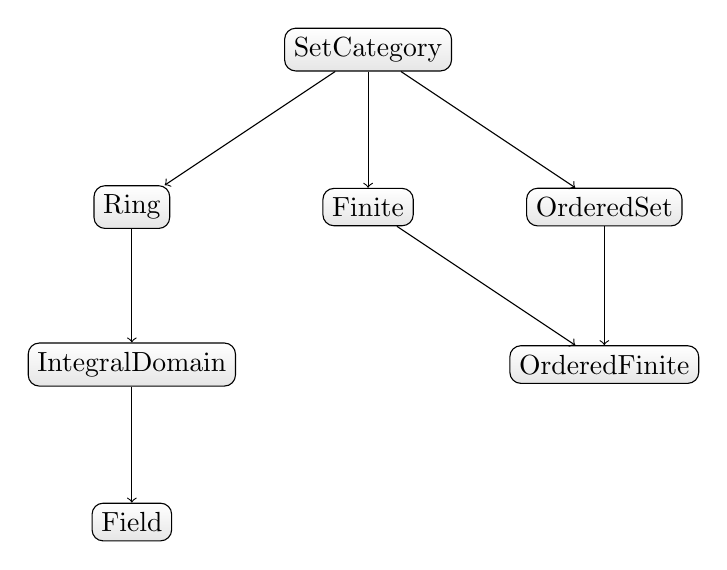
\begin{tikzpicture}[every node/.style = {shape=rectangle, rounded corners,
        draw, align=center, top color=white, bottom color=gray!20}]]
      \node(SetCategory) at (3,6) {\spadtype{SetCategory}};
      \node(Ring) at (0,4) {\spadtype{Ring}};
      \node(IntegralDomain) at (0,2) {\spadtype{IntegralDomain}};
      \node(Field) at (0,0) {\spadtype{Field}};
      \node(Finite) at (3,4) {\spadtype{Finite}};
      \node(OrderedSet) at (6,4) {\spadtype{OrderedSet}};
      \node(OrderedFinite) at (6,2) {\spadtype{OrderedFinite}};

      \draw[->](SetCategory)--(Ring);
      \draw[->]               (Ring)--(IntegralDomain);
      \draw[->]                       (IntegralDomain)--(Field);

      \draw[->](SetCategory)--(Finite);
      \draw[->]               (Finite)--(OrderedFinite);

      \draw[->](SetCategory)--(OrderedSet);
      \draw[->]               (OrderedSet)--(OrderedFinite);
    \end{tikzpicture}
  \end{center}
  \caption{A simplified category hierarchy.\label{fig:techintro-1}}
\end{figure}
%\horizontalline
\vskip .5\baselineskip
\end{texonly}
\begin{htonly}
\beginImportant
\begin{verbatim}
SetCategory +---- Ring       ---- IntegralDomain ---- Field
            |
            +---- Finite     ---+
            |                    \
            +---- OrderedSet -----+ OrderedFinite
\end{verbatim}
\begin{center}
Figure 1.  A  simplified category hierarchy.
\end{center}
\endImportant
\end{htonly}


\newpage

%------------------------------------------------------------------------------
\pseudoSection{Domains Belong to Categories by Assertion}
%------------------------------------------------------------------------------

\par %\noindent
A category designates a class of domains.
Which domains?
You might think that \spadtype{Ring} designates the class of all
domains that export
\spad{0}, \spad{1},
\spadopFrom{+}{Integer}, \spadopFrom{-}{Integer}, and
\spadopFrom{*}{Integer}.
But this is not so.
Each domain must {\it assert} which categories it belongs to.

The {\tt Export} part of the definition for \spadtype{Integer}
reads, for example:

\begin{verbatim}
Join(OrderedSet, IntegralDomain,  ...) with ...
\end{verbatim}
This definition asserts that \spadtype{Integer} is
both an ordered set and an integral domain.
In fact, \spadtype{Integer} does not explicitly export constants
\spad{0} and \spad{1} and operations \spadopFrom{+}{Ring},
\spadopFrom{-}{Ring} and
\spadopFrom{*}{Ring} at all: it inherits them all from \spad{Ring}!
Since \spadtype{IntegralDomain} is a descendant of \spad{Ring},
\spadtype{Integer} is therefore also a ring.

Assertions can be conditional.
For example, \spadtype{Complex(R)} defines its exports by:

\begin{verbatim}
Ring with ... if R has Field then Field ...
\end{verbatim}
Thus \spadtype{Complex(Float)} is a field but \spadtype{Complex(Integer)}
is not since \spadtype{Integer} is not a field.

You may wonder:
``Why not simply let the set of operations determine
whether a domain belongs to a given category?''.
\Language{} allows operation names (for example,
\spadfun{norm}) to have very different
meanings in different contexts.
The meaning of an operation in \Language{} is determined by context.
By associating operations with categories, operation names can be reused
whenever appropriate or convenient to do so.
As a simple example, the operation \spadop{<} might be used to denote
lexicographic-comparison in an algorithm.
However, it is wrong to use the same \spadop{<} with this
definition of absolute-value: {\tt abs(x) == if x < 0 then -x
else x.}
Such a definition for {\tt abs} in \Language{} is protected by context:
argument \spad{x} is required to be a
member of a domain of category \spadtype{OrderedSet}.

%------------------------------------------------------------------------------
\pseudoSection{Packages Are Clusters of Polymorphic Operations}
%------------------------------------------------------------------------------

\par %\noindent
In \Language{}, facilities for symbolic integration, solution of equations, and the like
are placed in ``packages''.
A {\it package}
\index{package}
is a special kind of domain: one whose exported operations
depend solely on the parameters of the constructor and/or
explicit domains.

If you want to use \Language{}, for example, to define some algorithms for solving
equations of polynomials over an arbitrary field \spad{F}, you
can do so with a package of the form:

\begin{verbatim}
MySolve(F: Field): Exports == Implementation
\end{verbatim}

where {\tt Exports} specifies the \spadfun{solve} operations you wish to
export and {\tt Implementation} defines functions for implementing your algorithms.
Once \Language{} has compiled your package, your algorithms can then be used
for any \spad{F}: floating-point numbers, rational numbers, complex
rational functions, and power series, to name a few.

% I think you need to talk somewhere about function implementations.
% You can also mention alternative implementations based on "has"
% conditionals.

%------------------------------------------------------------------------------
\pseudoSection{The Interpreter Builds Domains Dynamically}
%------------------------------------------------------------------------------

\par %\noindent
The \Language{} interpreter reads user input then builds whatever types
it needs to perform the indicated computations.
For example, to create the matrix
\begin{texonly}
\[M = \begin{pmatrix}x^2+1&0\\0&x / 2\end{pmatrix}\]
\end{texonly}
\begin{htonly}
\spad{M = [[x^2+1,0],[0,x / 2]]}
\end{htonly}
the interpreter first loads the
modules \spadtype{Matrix}, \spadtype{Polynomial}, \spadtype{Fraction},
and \spadtype{Integer} from the library, then builds the {\it domain tower}
``matrices of polynomials of rational numbers (fractions of integers)''.
% also, categories get loaded plus auxiliary domains
%\footnote{Most systems are preloaded with such common types; once
%modules are loaded they are immediately available to the interpreter.}

Once a domain tower is built, computation proceeds by calling operations
down the tower.
% "down the tower" is confusing
For example, suppose that the user asks to square the above matrix.
To do this, the function \spadopFrom{*}{Matrix} from \spadtype{Matrix}
is passed \spad{M} to compute \spad{M * M}.
The function is also passed
an environment containing \spad{R} that, in this case, is
\spadtype{Polynomial (Fraction (Integer))}.
This results in the successive calling of the \spadopFrom{*}{Fraction}
operations from \spadtype{Polynomial}, then from \spadtype{Fraction}, and
then finally from \spadtype{Integer} before a result is passed back up
the tower.

Categories play a policing role in the building of domains.
Because the argument of \spadtype{Matrix} is required to be
a ring, \Language{} will not build nonsensical types such as
``matrices of input files''.

%------------------------------------------------------------------------------
\pseudoSection{\Language{} Code is Compiled}
%------------------------------------------------------------------------------

\par %\noindent
\Language{} programs are statically compiled to machine code,
then placed into library modules.
Categories provide an important role in obtaining efficient object code by enabling:
\begin{itemize}
\item static type-checking at compile time;
\item fast linkage to operations in domain-valued parameters;
\item optimization techniques to be used for partially specified types
(operations for ``vectors of \spad{R}'', for instance, can be open-coded even
though \spad{R} is unknown).
\end{itemize}

%------------------------------------------------------------------------------
\pseudoSection{\Language{} is Extensible}
%------------------------------------------------------------------------------

\par %\noindent
Users and system implementers alike use the \Language{} language
to add facilities to the \Language{} library.
The entire \Language{} library is in fact written in the \Language{}
source code and available for user modification and/or extension.

\Language{}'s use of abstract datatypes clearly separates the exports
of a domain (what operations are defined) from its implementation (how
the objects are represented and operations are defined).
Users of a domain can thus only create and manipulate objects through
these exported  operations.
This allows implementers to ``remove and replace''
parts of the library safely by newly upgraded (and, we hope, correct)
implementations without consequence to its users.

Categories protect names by context,
making the same names available for use in other contexts.
Categories also provide for code-economy.
Algorithms can be parameterized categorically
to characterize their correct and most general context.
Once compiled, the same machine code is applicable
in all such contexts.

Finally, \Language{} provides an automatic, guaranteed interaction between
new and old code.
For example:
\begin{itemize}
\item if you write a new algorithm that requires a parameter to be a
field, then your algorithm will work automatically with every field
defined in the system; past, present, or future.
\item if you introduce a new domain constructor that produces a field,
then the objects of that domain can be used as parameters to any algorithm
using field objects defined in the system; past, present, or future.
\end{itemize}

These are the key ideas.
For further information, we particularly recommend your reading
chapters 11, 12, and 13, where these ideas are explained
in greater detail.
  % This ha no chapter number.

\part{Basic Features of \Language{}}
%
\input{ug01}
\input{ug02}
\input{ug03}
\input{ug04}
\input{ug05}
\input{ug06}

%--rhx: TODO:
% Unfortunately ug07 uses \item[\spadfun{foo}] which doesn't work
% since \spadfun has a verbatim-like argument. Fortunately, that only
% happens inside the description environment. So we simply redefine it
% for this chapter. Better rewrite the text in ug07.
\begingroup
\let\spaddescriptionsave\description
\def\description{\def\spadfun{\textspadfun}\spaddescriptionsave}
\input{ug07}
\endgroup

\part{Advanced Problem Solving and Examples}
%
\input{ug08}
\input{ug09}

\part{Advanced Programming in \Language{}}
%
\input{ug10}
\input{ug11}
\input{ug12}
\input{ug13}
\input{ug14}
\input{ug15}
%
\appendix

\input{ug16}
%\input{ug17}
%\input{ug18}
%\input{ug19}
%\input{ug20}
\input{ug21}
%
\printindex
\end{document}
